\chapter{Summary of impacts \\ 
% \small{\textit{-- Author Name}}
\index{Summary of impacts}
\label{Chapter::Summaryofimpacts}} 
\section{Operational impacts \label{Section::Operationalimpacts}}
\begin{enumerate}
    \item Centralized inventory control: The ability to manage inventory across multiple stores in a centralized manner will lead to greater efficiency and accuracy in inventory tracking and management.

    \item Mobile access: The ability to access inventory data and perform inventory management tasks remotely will increase flexibility and enable more efficient use of staff time.

    \item Customizable alerts: The ability to receive alerts for low inventory levels, stockouts, and other inventory-related issues will improve inventory management and reduce the risk of stockouts and overstocking.

    \item Integration with POS system: The integration of the inventory management system with the point-of-sale system will ensure that inventory levels are automatically updated based on sales transactions, reducing errors and improving accuracy.

    \item Vendor management: The inclusion of vendor management functionality will streamline the purchasing process and improve vendor relationships, leading to more timely delivery of goods and better inventory management.
\end{enumerate}
\section{Organizational impacts \label{Section::Organizationalimpacts}}
\begin{enumerate}
    \item Improved inventory accuracy: The proposed system's automatic updates and centralized inventory control will improve inventory accuracy, reducing errors related to manual data entry and providing more accurate inventory data.

    \item Increased efficiency: Mobile access, customizable alerts, and vendor management functionality will increase the efficiency of inventory management tasks, allowing store managers and staff to manage inventory more quickly and easily.

    \item Reduced costs: Improved inventory accuracy and efficiency will reduce costs associated with overstocking, stockouts, and other inventory-related issues. Additionally, vendor management functionality can help optimize the purchasing process and reduce costs associated with late or incorrect deliveries.
\end{enumerate}

\section{Impacts during development \label{Section::Impactsduringdevelopment}}
\begin{enumerate}
    \item Time and resource requirements: Developing the proposed system will require a significant investment of time and resources, including software development, hardware procurement, and staff training.

    \item Potential disruptions to current operations: The development process may disrupt current inventory management processes, especially if the new system requires changes to existing workflows or data management practices.

    \item Collaboration and communication: Developing the proposed system will require collaboration and communication between developers, project managers, store managers, and other stakeholders to ensure that the system meets their needs and is properly integrated into their workflows.

    \item Technical challenges: The development process may encounter technical challenges, including software bugs, hardware failures, or integration issues with other systems.
\end{enumerate}

\noindent
The technical challenges can be tracked and planned around by utilizing a Bug reporting and job management software. We propose the use of JIRA.
\begin{figure}[H]
  \centering
   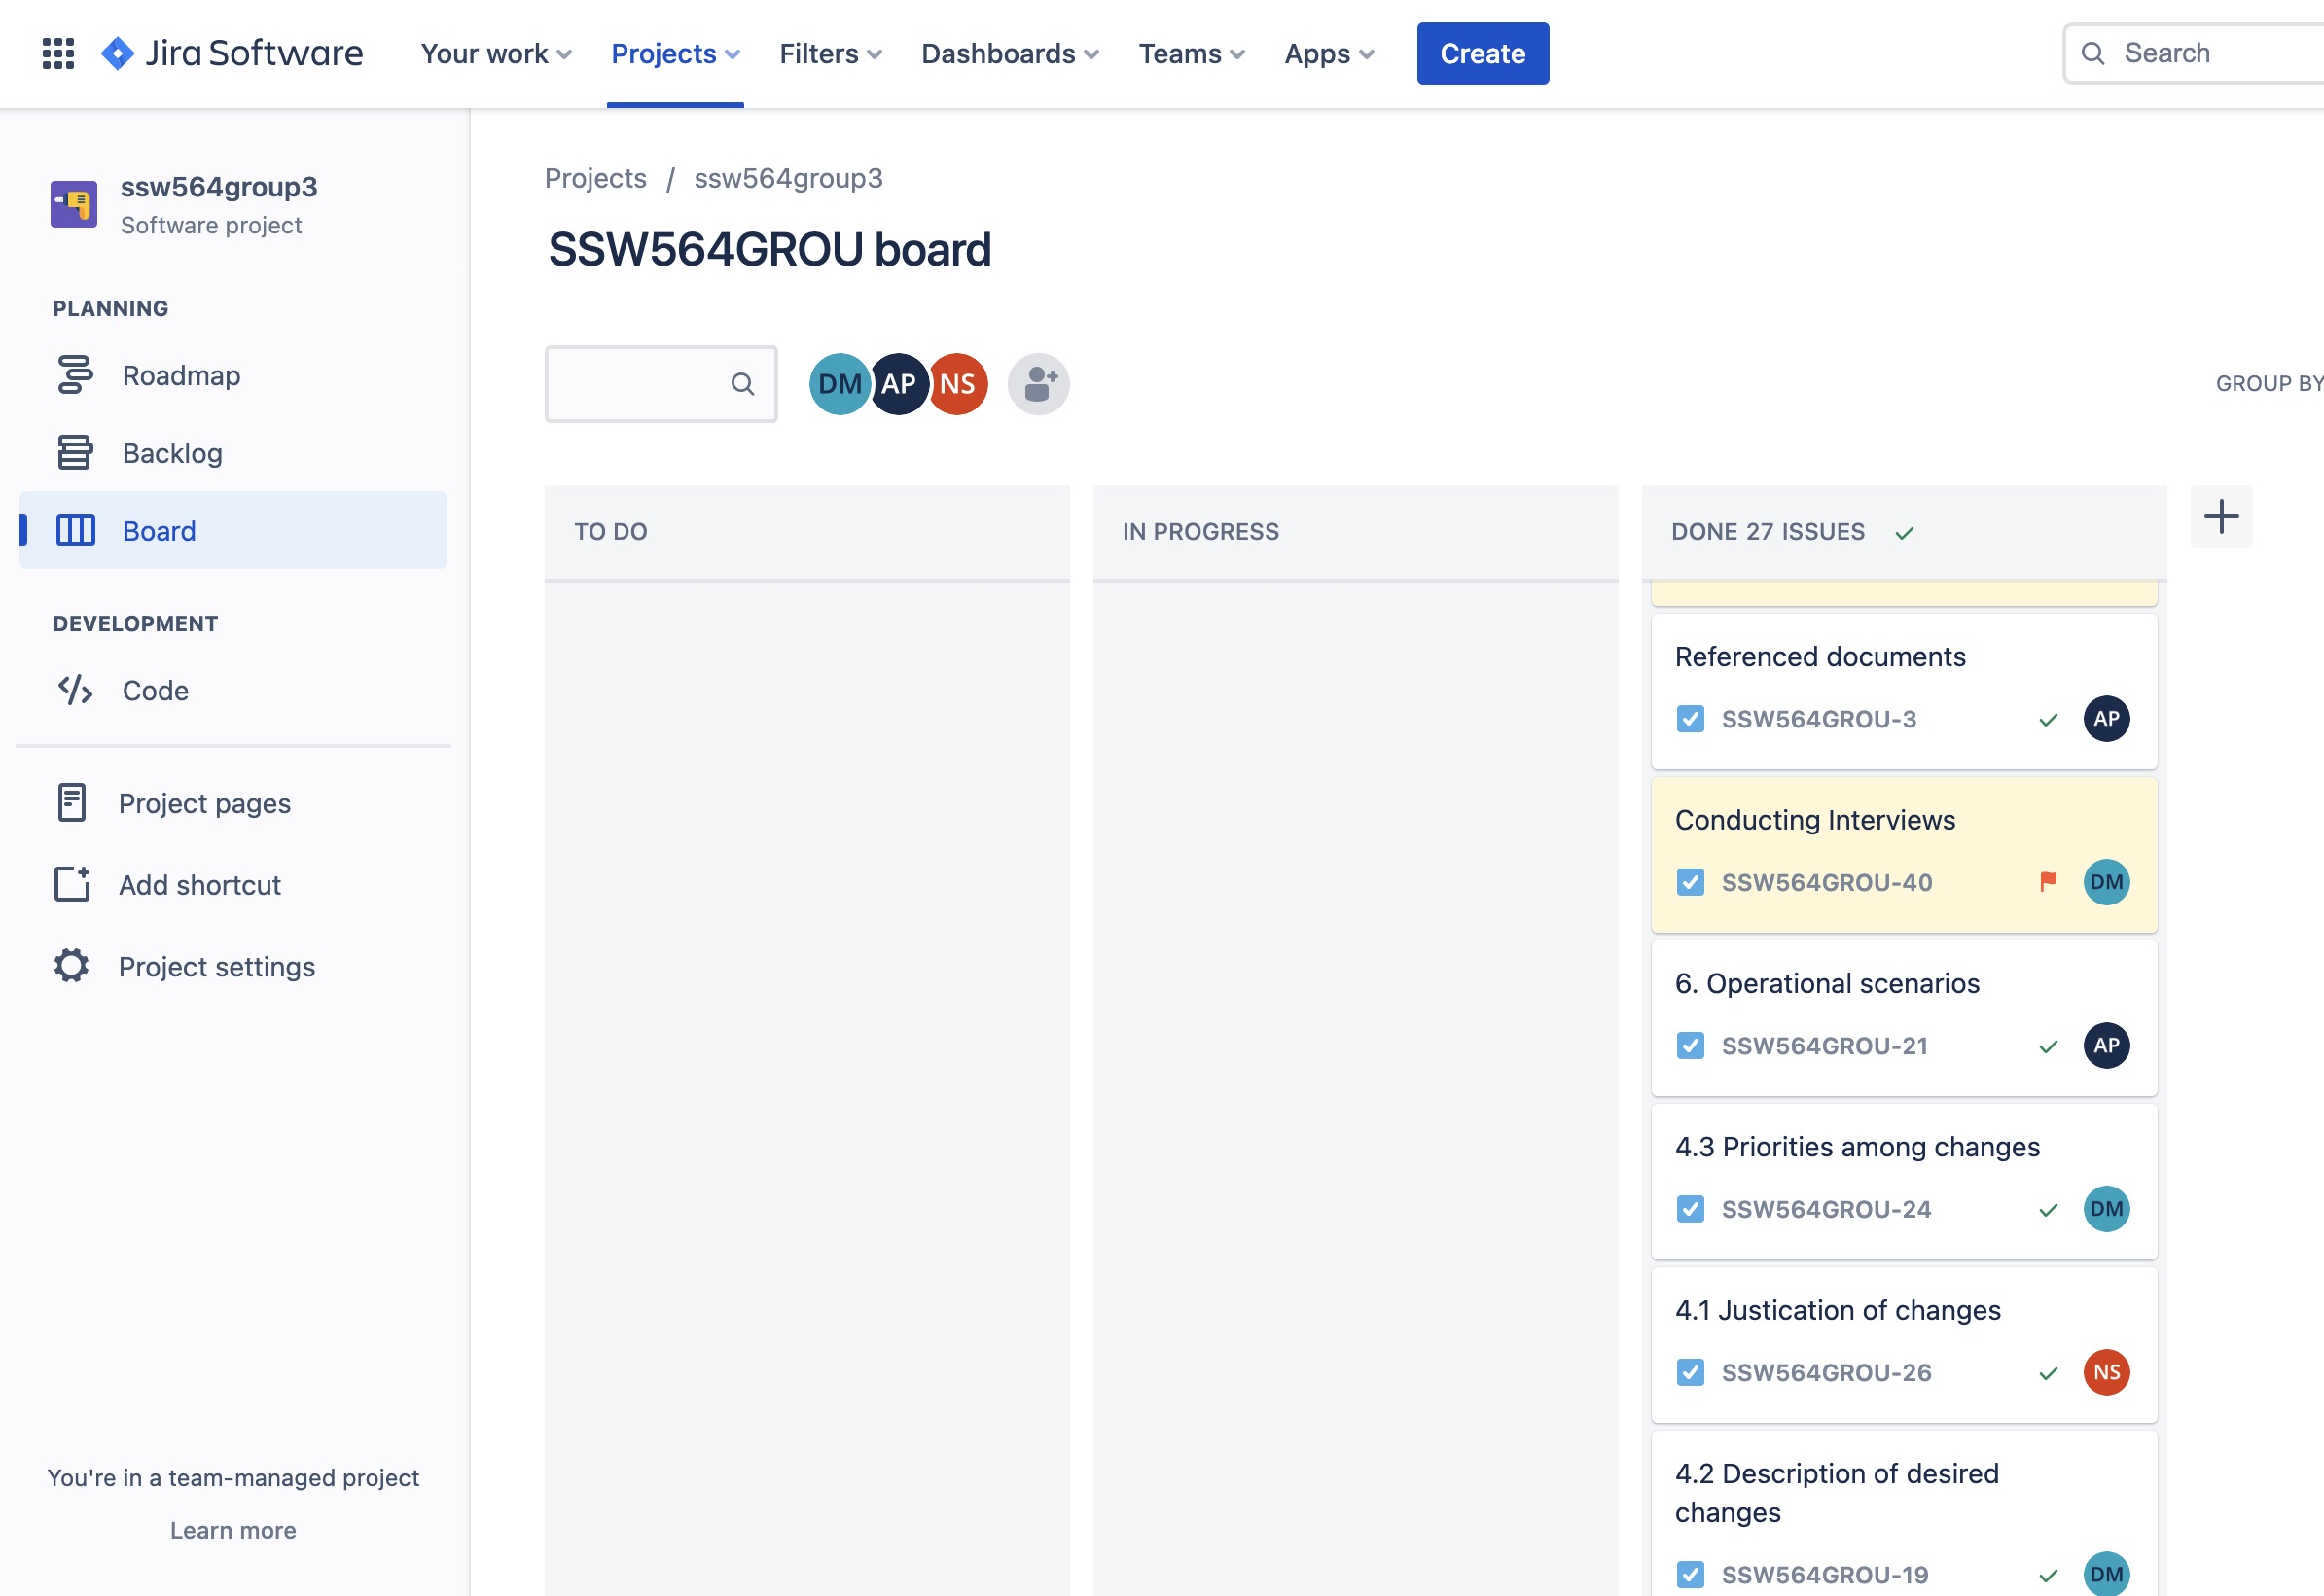
\includegraphics[width=9cm]{Figures/0DA589D3-1556-4FB9-9B0C-23CCDA029EBB_1_201_a.jpeg}
  \caption{Jira Homepage created for the project}
\label{}
\end{figure}
\newpage